\section{Supplementary Material}
\label{sec:appendix}


\begin{figure}
    \centering
    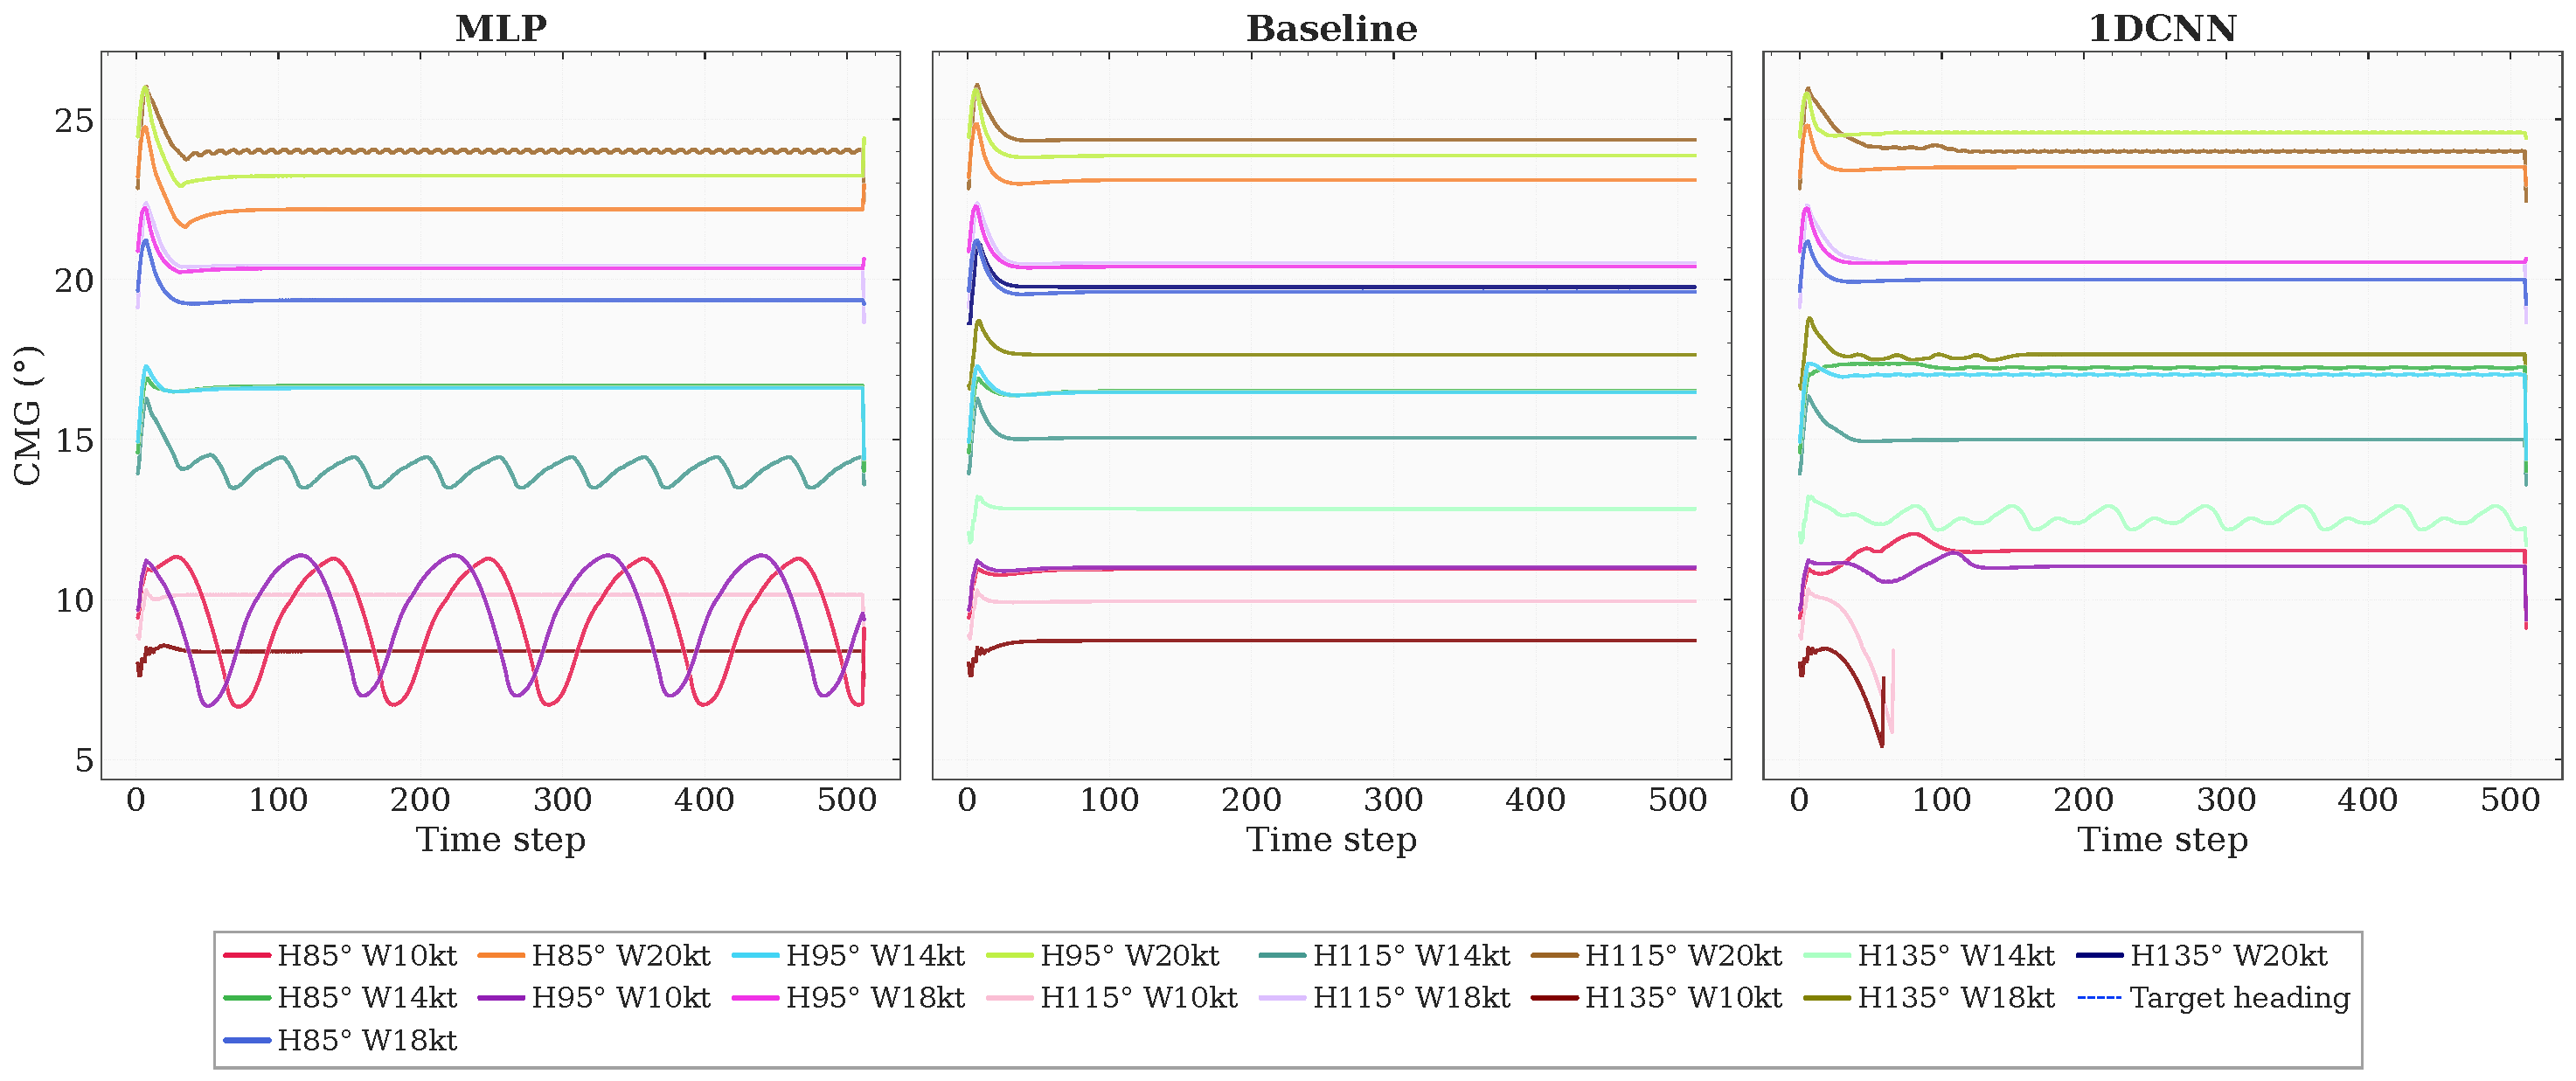
\includegraphics[width=1\linewidth]{resources/img/appendix/cmg_timeseries_pub.pdf}
    \caption{Caption}
    \label{fig:placeholder}
\end{figure}






%%% ENV
\begin{table}[h!]
\centering
\caption{Key Environmental and Simulation Parameters}
\label{table:env_params}
\begin{tabular}{ll p{8cm}}
\hline
\textbf{Section} & \textbf{Parameter} & \textbf{Description} \\ \hline
Global & \texttt{targetFrequency} & Defines the frequency (time step) of the simulation per environment step. \\
& \texttt{actionParam} & Magnitude of the target offset increment (fixed at 1$^\circ$). \\
& \texttt{deadStepNb} & Number of stabilization steps performed after an environment reset. \\
& \texttt{renderMode} & Visualization settings: \textit{human} (real-time) or \textit{human\_fast}. \\ \hline
Boat & \texttt{maxRudderAngle} & Maximum allowable deflection for the rudder control. \\
& \texttt{autoSetSail} & Real-time automatic sail adjustment based on wind conditions. \\ \hline
Wind/Waves & \texttt{wind\_speeds} & Sampling domain or fixed values for wind magnitude in knots. \\
& \texttt{swellGeneration} & Toggle for simulating external wave/swell perturbations. \\ \hline
Target & \texttt{target\_headings} & The primary heading objective for the underlying autopilot. \\ \hline
\end{tabular}
\end{table}
